\documentclass[a4paper,12pt,landscape]{article}
\usepackage[T1]{fontenc}
\usepackage[utf8]{inputenc}
\usepackage[francais]{babel}
\usepackage{amsfonts}
\usepackage[margin=2.5cm]{geometry}
\usepackage{graphicx}
\usepackage{subfig}
\usepackage{array}
%\usepackage{wrapfigure}

\begin{document}
\title{Projet EDMO}
\author{Annie Cathignol\\Louis Becquey\\3-BIM}
\date{\today}
\maketitle

\begin{center}
\begin{figure}[b!]

\includegraphics[height=3.2cm]{InsaBioLogo3.png}
\end{figure}
\end{center}

\newpage

\section{Questions de Cours}
\subsection{Résultat 1}
{\it \bf Pour toute fonction f assez régulière (de classe $C^{p}$ ), le schéma explicite à un pas est consistant d’ordre p avec le problème de Cauchy correspondant si:}\\
\begin{center}
$\Phi (t,x,0) = f(t,x)$ ,  \\
$\frac{\partial \Phi}{\partial h} (t,x,0) = \frac{1}{2}Df(t,x)$ , \\
$\vdots$ \\
$\frac{\partial^{p-1}\Phi}{\partial h^{p-1}} (t,x,0) = \frac{1}{p}D^{p-1}f(t,x)$ , \\
\end{center}


\subsection{Résultat 2}
{\it \bf Pour qu’un schéma de Runge-Kutta explicite à un pas soit au-moins d’ordre 2, il faut et il suffit que les points $b_{i}$, les poids intermédiaires $a_{i,j}$ et les paramètres $c_{i}$ (i, j variant de 1 à s) vérifient:} $$\sum_{i=1}^{s}b_{i}c_{i} = \frac{1}{2} \; \textrm{   d'une part, et d'autre part   } \; \sum_{i=1}^{s}b_{i}(\sum_{j=1}^{i-1}a_{i,j})= \frac{1}{2}$$


\section{Exercice 1 - Problème raide}
On considère le problème de Cauchy suivant :
trouver $u \in C^{1}([0,1], \mathbb{R} )$ telle que
$$
(C) \left \{
\begin{array}{l}
	u'(t)= -150u(t) + 30 \\
	u(0) = 1
\end{array}
\right.
$$
\newpage
\subsection{}
Il s'agit d'une équation différentielle linéaire d'ordre 1, avec second membre, on peut trouver une solution exacte en procédant comme suit:\\
Partons de l'équation $$u' + 150u = 30$$
Multiplions chaque terme par $e^{150t}$ : $$u'.e^{150t}+150.e^{150t}.u = 30.e^{150t}$$
$$(u.e^{150t})'=30.e^{150t}$$
Intégrons entre 0 et t ($t \in [0,1]$): $$\int_{0}^{t}(u_{(s)}.e^{150s})'.ds = \int_{0}^{t}30.e^{150s}.ds$$
$$u_{(t)}.e^{150t}-u_{(0)} = {\left [ \frac{1}{5}e^{150s} \right ]}_{0}^{t}= \frac{1}{5}e^{150t}-\frac{1}{5}$$
$$u_{(t)} = { \left ( \frac{e^{150t}+4}{5} \right ) }e^{-150t}$$
$$u_{(t)} = \frac{1}{5}+\frac{4}{5}e^{-150t}$$
Cette fonction u est bien définie sur l'intervalle [0,1], vérifions qu'elle est bien solution du problème (C):\\

$u_{(0)}= \frac{1}{5}+\frac{4}{5}=\frac{5}{5}=1 \Rightarrow $ OK\\

$u'_{(t)}= -120e^{-150t}$\\

$-150 u_{(t)} +30 = -150{ \left( \frac{1}{5}+\frac{4}{5}e^{-150t} \right) } +30 = -30 -120e^{-150t} +30 = u'_{(t)} \Rightarrow $OK\\

Donc on a bien une solution exacte au problème de Cauchy.

On a donc quand $t \rightarrow \infty$, 
$$\lim_{t \rightarrow +\infty}u_{(t)}=\frac{1}{5}+\frac{4}{5} { \left( \lim_{t \rightarrow +\infty}e^{-150t} \right ) }= \frac{1}{5}.$$

\subsection{}
Considérons le schéma d'Euler explicite pour ce problème de Cauchy:
$$\left \{
\begin{array}{l}
	u_{n+1}= u_{n} + h f(t_n , u_n)\\
	u_0 = 1
\end{array}
\right.
\Leftrightarrow
\left \{
\begin{array}{l}
	u_{n+1}= u_{n} + h(-150 u_n + 30)\\
	u_0 = 1
\end{array}
\right.
\Leftrightarrow
\left \{
\begin{array}{l}
	u_{n+1}= (1-150h)u_{n} + 30h\\
	u_0 = 1
\end{array}
\right.$$
On peut écrire une relation de récurrence entre $u_{n+1}-\frac{1}{5}$ et $u_{n}-\frac{1}{5}$:
$$u_{n+1}-\frac{1}{5}= u_n - 150hu_n+30h-\frac{1}{5}= (u_n-\frac{1}{5})-150hu_n + 30h = (u_n-\frac{1}{5})-150h(u_n-\frac{1}{5})$$
$$(u_{n+1}-\frac{1}{5})= (u_n-\frac{1}{5})(1-150h)$$
Cette relation permet d'exprimer $u_n$ en fonction de n et h:\\
Soit $x_n=u_{n}-\frac{1}{5}$, on a $x_{n+1}=(1-150h)x_n$, donc par exemple $x_1=(1-150h).x_0$, puis $x_2=(1-150h)^2.x_0$, et on peut montrer par récurrence que, pour $n \in \mathbb{N}^*$,
$$x_n=(1-150h)^n.x_0$$
D'où $(u_n-\frac{1}{5})=(1-150h)^n(u_0-\frac{1}{5})$, et comme $u_0=1$:
$$u_n=\frac{4}{5}(1-150h)^n+\frac{1}{5}$$
Si l'on suppose ensuite $h=1/50$ constant, on peut ré-écrire l'expression précédente sous la forme: $$u_n=\frac{4}{5}(-2)^n+\frac{1}{5}$$ On constate que la limite de $u_n$ quand $t \rightarrow \infty$ n'existe pas avec ce schéma.\\
On peut donc en conclure que ce schéma d'Euler explicite n'est pas  asymptotiquement stable: Lorsqu'on fait de plus en plus d'itérations, on ne se rapproche pas de la solution exacte.

\subsection{}
Considérons donc plutôt un schéma d'Euler implicite {\it (On rappelle que comme h>0, (1+150h)>0 )}
$$\left \{
\begin{array}{l}
	u_{n+1}= u_{n} + h f(t_{n+1} , u_{n+1})\\
	u_0 = 1
\end{array}
\right.
\Leftrightarrow
\left \{
\begin{array}{l}
	u_{n+1}= u_{n} + h(-150 u_{n+1} + 30)\\
	u_0 = 1
\end{array}
\right.$$
$$\begin{array}{l}
	u_{n+1}=u_n - 150h u_{n+1} + 30h\\
	(150h +1)u_{n+1} = u_n + 30h\\
\end{array}
\Leftrightarrow
u_{n+1}=\frac{u_n+30h}{(1+150h)}$$
Cette fois, la relation de récurrence entre $u_{n+1}-\frac{1}{5}$ et $u_{n}-\frac{1}{5}$ donne:
$$(u_{n+1}-\frac{1}{5})=\frac{u_n+30h}{(1+150h)}-\frac{1}{5}=\frac{5(u_n+30h)-(1+150h)}{5(1+150h)}=\frac{(u_n+30h)-(\frac{1}{5}+30h)}{(1+150h)}=\frac{u_n+30h-\frac{1}{5}-30h}{(1+150h)}=\frac{(u_n-\frac{1}{5})}{(1+150h)}$$
Posons $x_n=u_{n}-\frac{1}{5}$, on a alors $x_{n+1}=x_n/(1+150h)$, donc par exemple $x_1=x_0/(1+150h)$, puis $x_2=x_0/(1+150h)^2$, et on peut montrer par récurrence que, pour $n \in \mathbb{N}^*$,
$$x_n=x_0/(1+150h)^n$$
D'où $(u_n-\frac{1}{5})=\frac{(u_0-\frac{1}{5})}{(1+150h)^n}$, et comme $u_0=1$:
$$u_n=\frac{4}{5}\frac{1}{(1+150h)^n}+\frac{1}{5}$$
Si l'on suppose ensuite $h=1/50$ constant, on peut ré-écrire l'expression précédente sous la forme: $$u_n=\frac{4}{5*4^n}+\frac{1}{5}$$
Cette fois, on peut écrire que $$\lim_{n \rightarrow +\infty}u_n = \frac{1}{5}\lim_{n \rightarrow +\infty}{ \left( \frac{1}{4^{n-1}} \right) }+\frac{1}{5}=\frac{1}{5}$$
Cette fois, on peut donc conclure que lorsqu'on augmente le nombre d'itérations, on converge vers la valeur numérique de la solution exacte: ce schéma d'Euler implicite est donc asymptotiquement stable.


\section{Exercice 2 - Une mise en jambe pour la programmation}

On considère le problème de Cauchy suivant :
trouver y définie sur [0,4] telle que
$$
(C2) \left \{
\begin{array}{l}
	y'(t)= 4e^{0.8t}-0.5y(t) \\
	y(0) = 2
\end{array}
\right.
$$
\subsection{}
On a un problème de Cauchy y'=f(t,y) où f(t,y) est continue sur $\mathbb{R}^2$: $f(t,y)=4e^{0.8t}-0.5y$. Cette même fonction est localement lipschitzienne par rapport à sa variable y, puisqu'elle est de classe $C^1$ dans [0,4].\\
Donc selon le théorème de Cauchy-Lipschitz, on a existence, unicité et régularité d'une solution y(t) définie sur au moins [0,4].\\

Cherchons la solution exacte du problème: il s'agit d'une équation différentielle linéaire du premier ordre avec second membre. Procédons comme suit:
$$y'+0.5y=4.e^{0.8t}$$
Multiplions chaque terme par $e^{0.5t}$ : $$(e^{0.5t}.y(t))'=4e^{1.3t}$$
Intégrons entre 0 et t: $${\left[ e^{0.5s}.y(s) \right]}^t_0={\left[ \frac{4}{1.3}e^{1.3s} \right]}^t_0$$
$$e^{0.5t}.y(t)-y(0)=\frac{4}{1.3}e^{1.3t}-\frac{4}{1.3}$$
$$y(t)={\left( \frac{4}{1.3}e^{1.3t}-\frac{4}{1.3}+2 \right)}e^{-0.5t}$$
$$y(t)=\frac{4}{1.3}e^{0.8t}+{\left( 2-\frac{4}{1.3} \right) }e^{-0.5t}$$
$$y(t)=\frac{4}{1.3}e^{0.8t} -\frac{1.4}{1.3} e^{-0.5t}$$
Cette fonction y est bien définie sur [0,4], et on a bien $y(0)=2$.

\subsection{}
Considérons le schéma d'Euler explicite associé à ce problème {\it (On a h=1)}:
$$\left \{
\begin{array}{l}
	y_{n+1}= y_n + h f(t_n,y_n)\\
	y_0 = 2
\end{array}
\right.
\Leftrightarrow
\left \{
\begin{array}{l}
	y_{n+1}= y_n + 4e^{0.8t_n}-0.5y_n\\
	y_0 = 2
\end{array}
\right.
\Leftrightarrow
\left \{
\begin{array}{l}
	y_{n+1}= 0.5y_n + 4e^{0.8t_n}\\
	y_0 = 2
\end{array}
\right.$$
\paragraph{A l'ordre 1}
Ici, $\Phi(t,y,h)$=f(t,y) qui est lipschitzienne par rapport à sa deuxième variable. Donc $\Phi$ est lipschitzienne par rapport à sa deuxième variable, donc le schéma est stable à l'ordre 1.\\
De plus, comme $\Phi(t,y,h)$=f(t,y) on a $\Phi(t,y,0)$=f(t,y), donc le schéma est consistant d'ordre 1 avec le problème de Cauchy.\\

Donc par le théorème de LAX, le schéma est convergent d'ordre au moins 1 vers la solution du problème de Cauchy.

\paragraph{A l'ordre 2}
Ici, $\Phi(t,y,h)$ est de classe $C^2$. Donc $\Phi$ est lipschitzienne par rapport à sa deuxième variable, donc le schéma est stable à l'ordre 2 également.\\
Cette fois par contre, $\frac{\partial \Phi}{\partial h} (t,y,0)=0 \neq \frac{1}{2}Df(t,y)$, donc le schéma n'est pas consistant à l'ordre 2.\\
%\begin{wrapfigure}[1]{r}{10cm}
%	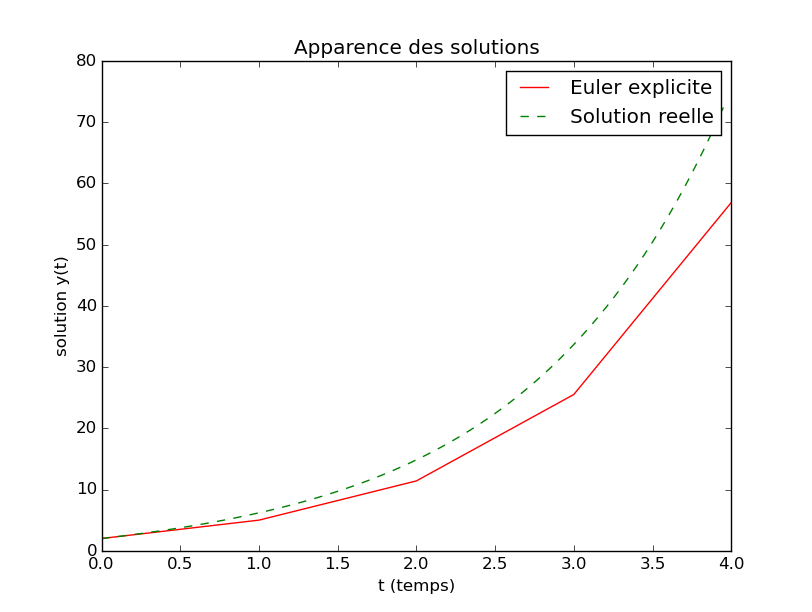
\includegraphics[scale=0.45]{ex2.png}
%	\caption{Comparaison entre méthode numérique et solution réelle sur l'intervalle [0,4]}
%\end{wrapfigure}
Donc le schéma n'est convergent que d'ordre 1.

\subsection{}

Avec ce schéma (Euler explicite), nous obtenons les résultats suivants:\\
L'erreur reste élevée (converge vers 24.66\%), et on voit bien que\\ le schéma n'est pas asymptotiquement convergent.

\begin{table}[h]
\hspace{2cm}
\begin{tabular}{|c|c|c|c|}
\hline
	$t_i$ & $y(t_i)$ & $y_i$ & $\epsilon_i$ \\
\hline
	$t_0=0$ & $2$ & 2 & $10^{-14}\%$ \\
\hline
	$t_1=1$ & $\frac{4}{1.3}e^{0.8} -\frac{1.4}{1.3\sqrt{e}}\approx 6.19$ & $\approx 5$ & $19.3\%$ \\
\hline
	$t_2=2$ & $\frac{4}{1.3}e^{1.6} -\frac{1.4}{1.3e}\approx 14.84$ & $\approx 11.40$  & $23.2\%$ \\
\hline
	$t_3=3$ & $\frac{4}{1.3}e^{2.4} -\frac{1.4}{1.3e\sqrt{e}}\approx 33.68$& $\approx 25.51$ & $24.2\%$ \\
\hline
	$t_4=4$ & $\frac{4}{1.3}e^{3.2} -\frac{1.4}{1.3e^2}\approx 75.33$ & $ \approx 56.85$  & $24.5\%$ \\
\hline
\end{tabular}
\end{table}

\section{Exercice 3 - Comparaison entre plusieurs méthodes}
On considère le problème de Cauchy suivant pour $t\in [0,T]$:
$$
(C3) \left \{
\begin{array}{l}
	x'(t)= -tx(t) \\
	x(0) = x_0
\end{array}
\right.
$$
\subsection{}
On a un problème de Cauchy x'=f(t,x) où f(t,x) est continue sur $\mathbb{R}^2$: $f(t,x)=-tx$. Cette même fonction est localement lipschitzienne par rapport à sa variable x, puisqu'elle est de classe $C^1$ dans [0,T] comme dans tout $\mathbb{R}^2$.\\
Donc selon le théorème de Cauchy-Lipschitz, on a existence, unicité et régularité d'une solution x(t) définie sur au moins [0,T].\\

Cherchons la solution exacte du problème: il s'agit d'une équation différentielle du premier ordre à variables séparables. Ainsi,
$$\frac{x'}{x}=-t$$
$$\int_0^t\frac{x'_{(s)}}{x_{(s)}}.ds = - \int_0^t s.ds$$
$$ln(x_{(t)})-ln(x_0)=-\frac{1}{2}t^2$$
$$x(t)=x_0 e^{-\frac{1}{2}t^2}$$
Cette fonction est bien définie sur les intervalles positifs, et x(0) vaut bien $x_0$.
Vérifions:
$$x'(t)=-t x_0 e^{-\frac{1}{2}t^2}=-tx(t)$$
Donc il s'agit bien de la solution du problème de Cauchy.

\subsection{}
\subsubsection{Schéma d'Euler Explicite}
Considérons le schéma d'Euler explicite associé à ce problème {\it (On a h=0.3)}:
$$\left \{
\begin{array}{l}
	x_{n+1}= x_n + h f(t_n,x_n)\\
	x_0 
\end{array}
\right.
\Leftrightarrow
\left \{
\begin{array}{l}
	x_{n+1}= x_n -ht_nx_n\\
	x_0
\end{array}
\right.
\Leftrightarrow
\left \{
\begin{array}{l}
	x_{n+1}= (1-0.3t_n)x_n\\
	x_0
\end{array}
\right.$$
Ici, $\Phi(t,x,h)$=f(t,x) qui est lipschitzienne par rapport à sa deuxième variable. Donc $\Phi$ est lipschitzienne par rapport à sa deuxième variable, donc le schéma est stable.\\

\subsubsection{Schéma du point milieu}
Le schéma du point milieu associé \textit{(h vaut toujours 0.3)}:\\
$$\left \{
\begin{array}{l}
	x_{n+1}= x_n + h f(t_n+\frac{h}{2},x_n+\frac{h}{2}f(t_n,x_n))\\
	x_0 
\end{array}
\right.
\Leftrightarrow
\left \{
\begin{array}{l}
	x_{n+1}= x_n +0.3\left[ -\left( t_n+\frac{0.3}{2}\right) \left( x_n+\frac{0.3}{2}(-t_nx_n)\right) \right]\\
	x_0
\end{array}
\right.$$
$$\Leftrightarrow
\left \{
\begin{array}{l}
	x_{n+1}= x_n-0.3(t_n+0.15)(1-0.15t_n)x_n\\
	x_0
\end{array}
\right.
\Leftrightarrow
\left \{
\begin{array}{l}
	x_{n+1}= (1-0.3(t_n+0.15)(1-0.15t_n))x_n\\
	x_0
\end{array}
\right.$$
$\Phi(t,x,h)=-(t+\frac{h}{2})(x-\frac{h}{2}tx)$ est de classe $C^\infty$, donc suffisamment régulière. On la supposera donc lipschitzienne par rapport à sa deuxième variable, donc le schéma est stable.
\subsubsection{Schéma de Runge-Kutta-4}
Intéressons nous aussi au schéma de Runge-Kutta 4 associé à ce problème de Cauchy \textit{(h=0.3 constant)}:
$$\left \{
\begin{array}{l}
	x_0 \\
	X_1=x_n\\
	X_2=x_n-\frac{h}{2}t_nX_1\\
	X_3=x_n-\frac{h}{2}(t_n+\frac{h}{2})X_2\\
	X_4=x_n-h(t_n+\frac{h}{2})X_3\\
	x_{n+1}=x_n-h\left[\frac{1}{6}t_nX_1+\frac{1}{3}(t_n+\frac{h}{2})X_2+\frac{1}{3}(t_n+\frac{h}{2})X_3+\frac{1}{6}(t_n+h)X_4\right]
\end{array}
\right.
\left \{
\begin{array}{l}
	x_0 \\
	X_1=x_n\\
	X_2=x_n-0.15t_nx_n\\
	X_3=x_n-0.15(t_n+0.15)(x_n-0.15t_nx_n)\\
	X_4=x_n-0.3(t_n+0.15)(x_n-0.15(t_n+0.15)(x_n-0.15t_nx_n))\\
	x_{n+1}=x_n-0.3\left[\frac{1}{6}t_nX_1+\frac{1}{3}(t_n+0.15)X_2+\frac{1}{3}(t_n+0.15)X_3+\frac{1}{6}(t_n+0.3)X_4\right]
\end{array}
\right.$$\\
$\Phi(t,x,h)$ est un polynôme (de degré 1) par rapport à sa deuxième variable (x), donc $\Phi$ est suffisamment régulière. On la suppose lipschitzienne par rapport à sa deuxième variable, le schéma est donc stable.\\

\subsubsection{Ordre de consistance}
Pour déterminer l'ordre de consistance et de convergence, et pour nous éviter l'aspect calculatoire, on s'intéresse à la quantité $max | x(t_n) - x_n |$. On sait que le schéma converge à l'ordre p si et seulement si $max | x(t_n) - x_n | \leq Kh^p$.\\
Ainsi, la constante restant la même, $max | x(t_n) - x_n |$ varie comme $h^p$ quand h varie.\\

On se propose donc de calculer cette quantité $max | x(t_n) - x_n |$ en faisant varier le nombre N de points calculés dans l'intervalle [0,T]: On rappelle que le pas h est donné par $h=\frac{(T-0)}{N}$, donc $h^p=\frac{T^p}{N^p}$.\\

Les résultats observés pour les trois schémas sont réunis dans ce graphique:\\

\begin{table}[h!]
\begin{tabular}{cb{14cm}}
\subfloat[Erreur absolue maximale en fonction de N (échelle logarithmique)]{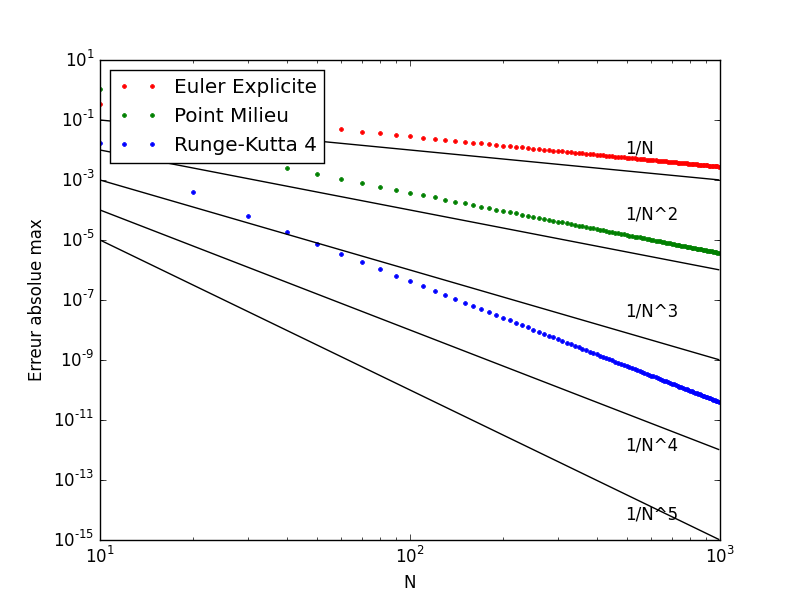
\includegraphics[scale=0.40]{ex3_erreur.png}}
\hspace{1cm}
&
\hspace{7mm} On remarque donc qu'à une constante près, $max | x(t_n) - x_n |$ varie comme $h^1$ pour le schéma d'Euler explicite, comme $h^2$ pour le schéma du point milieu, et comme $h^4$ pour le schéma de Runge-Kutta 4.
On peut donc dire que le schéma d'Euler explicite converge à l'ordre 1, celui du point milieu à l'ordre 2, et celui de Runge-Kutta converge à l'ordre 4.\vspace{1cm}
\\
\end{tabular}
\end{table}

\subsubsection{Stabilité asymptotique}
On applique le Test Linéaire Standard (TLS) aux schémas, et on observe le comportement asymptotique des trajectoires.

$$
(TLS)
\left \{
\begin{array}{l}
x'=-Lx\\
x(0)=x_0\\
\end{array}
\right.
$$
\begin{table}[h!]
\centering
\begin{tabular}{ccl}
\subfloat[Comportement asymptotique pour une condition (L,h)=(3,$\frac{1}{2}$) donnée]{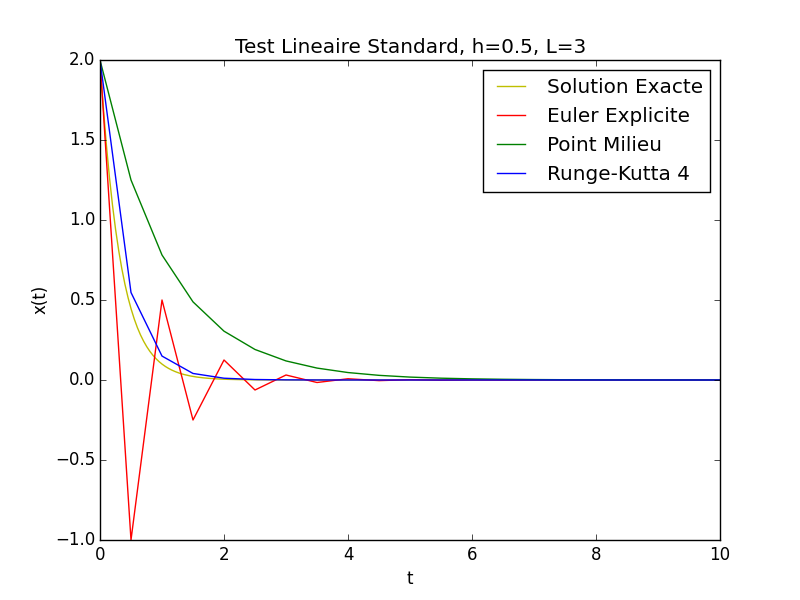
\includegraphics[scale=0.40]{ex3_TLS-1.png}}
&
\subfloat[Comportement asymptotique pour une autre condition (L=5)]{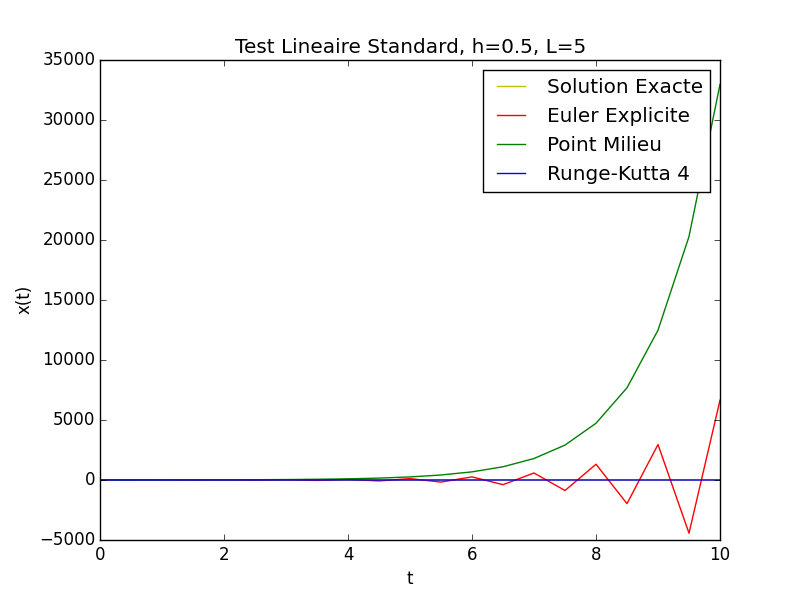
\includegraphics[scale=0.40]{ex3_TLS-2.png}}
&
\subfloat[Comportement asymptotique pour une autre condition (L=8,h=1)]{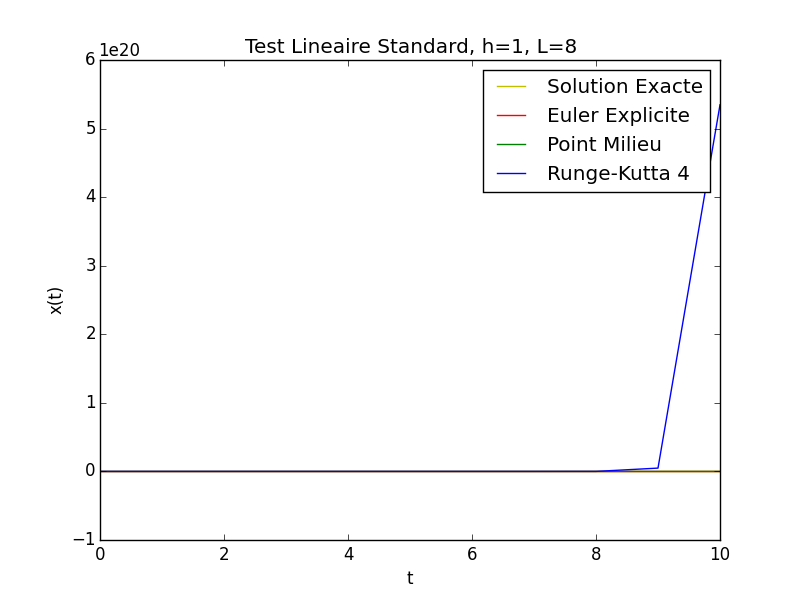
\includegraphics[scale=0.40]{ex3_TLS-3.png}}
\\
\end{tabular}
\end{table}

On voit que dans les 3 cas, h est soumis à conditions par rapport à L: Les schémas ne sont donc pas inconditionnellement stables. Cherchons les conditions sur h pour que le schéma soit A-stable:
\newpage
\paragraph{pour Euler Explicite:}
On obtient donc la suite $x_{n+1}=x_n-hLx_n=x_n(1-hL)$ donc on peut montrer par récurrence que $x_{n}=x_0 (1-hL)^{n}$. Le schéma est A-stable si $x_n$ tend vers 0 quand n tend vers l'infini, c'est à dire si et seulement si:\\
$$-1<1-hL<1$$
$$-2<-hL<0$$
$$0<hL<2$$
$$h<2/L$$ 
Le schéma n'est A-stable que pour $h<\frac{2}{L}$.


\paragraph{pour le Point Milieu:}
En procédant de la même façon, on obtient la suite $x_{n+1}=x_n(1-Lh+L^2h)$. Par récurrence, on peut montrer que $x_n=x_0(1-Lh+L^2h)^n$. Le schéma est donc A-stable uniquement si:
$$-1<1-Lh+L^2h<1$$
$$-2<-Lh+L^2h<0$$
$$-2<h(L^2-L)<0$$
h étant positif, la condition $h(L^2-L)<0$ n'est vraie que pour $L\in[0,1]$. Donc le schéma est A-stable pour $h<\frac{-2}{L^2-L}$ avec $L\in[0,1]$.

\paragraph{pour Runge-Kutta 4:}
La suite est plus complexe, mais le même principe peut être appliqué:\\ $x_{n+1}=x_n(1-\frac{hL}{6}(2-hL(1-\frac{h}{2}L(1-\frac{h}{2}L)))-\frac{hL}{3}(2-\frac{h}{2}L-\frac{h}{2}L(1-\frac{h}{2}L)))$ donc on peut écrire $x_n=x_0\times K(h,L)^n$ où $K(h,L)$ est un polynôme de degré 4, donc non entièrement inclus dans l'intervalle $[-1,1]$, donc la stabilité asymptotique est bien soumise à conditions sur h et L.


Donc les trois schémas ne sont pas inconditionnellement stables, on devra soit faire attention aux pas de temps h choisis, soit préférer utiliser un schéma implicite.

\subsection{}

\newpage
\section{Exercice 4 - Problème d'équation Proie-Prédateur}

On considère le problème de Cauchy du modèle de Lotka-Volterra, avec $y_1$ et $y_2$ définies sur $\mathbb{R}^+$:
$$
(PP)
\left \{
\begin{array}{l}
	y'_1(t)=1.2y_1-0.6y_1y_2\\
	y'_2(t)=-0.8y_2+0.3y_1y_2\\
	y_1(0)=2\\
	y_2(0)=1\\
\end{array}
\right.$$\\
\subsection{}

L'évolution des proies à chaque génération est la différence de l'augmentation naturelle des proies par reproduction (soit ici +$1.2y_1$), qui est toujours positive ou nulle, et du nombre de proies mangées pendant la génération (à cause des prédateurs).\\

La réponse fonctionnelle (\textit{le nombre de proies mangées par prédateur et par unité de temps}) est dépendante du nombre de proies. Ici elle est de $0,6y_1$ proies/prédateur/temps, c'est une réponse fonctionnelle de Holling de type I.\\

L'évolution des prédateurs est la diminution naturelle exponentielle s'il n'y a pas de proies (les prédateurs meurent par manque de nourriture), additionnée de l'influence positive qu'apporte l'interaction des populations Proies-Prédateurs aux prédateurs.\\

Donc $y_1$ représente la population de proies et $y_2$ celles des prédateurs.

\subsection{}

On programme la fonction suivante, qu'on résoudra avec le solveur \textit{ode45()} de MatLab:\\
 \\
 \\ 
\texttt{function yp=predprey(t,y)\\
yp=[1.2*y(1)-0.6*y(1)*y(2) ;-0.8*y(2)+0.3*y(1)*y(2)] ;}\\
 \\
\texttt{[t,y]=ode45(@predprey, tspan, y0);} permet donc de récupérer deux listes t et y grâce au solveur ode45() pour ensuite tracer un graphique des solutions.
De plus, comme la commande renvoie sous le nom 'y' un tableau de deux colonnes (pour $y_1$ et $y_2$), chaque colonne contenant la valeur de l'effectif de la population à l'instant t correspondant à la ligne, on a \texttt{y(:,1)} la liste des valeurs de $y_1$ au cours du temps, et \texttt{y(:,2)} celle des valeurs de $y_2$. Donc la commande \texttt{plot(y(:,1),y(:,2));} nous trace $y_2$ en fonction de $y_1$, c'est à dire le portrait de phases du système dynamique:

\begin{table}[h!]
\centering
\begin{tabular}{ccl}
\subfloat[Coévolution des populations de proies et prédateurs au cours du temps, en unités arbitraires]{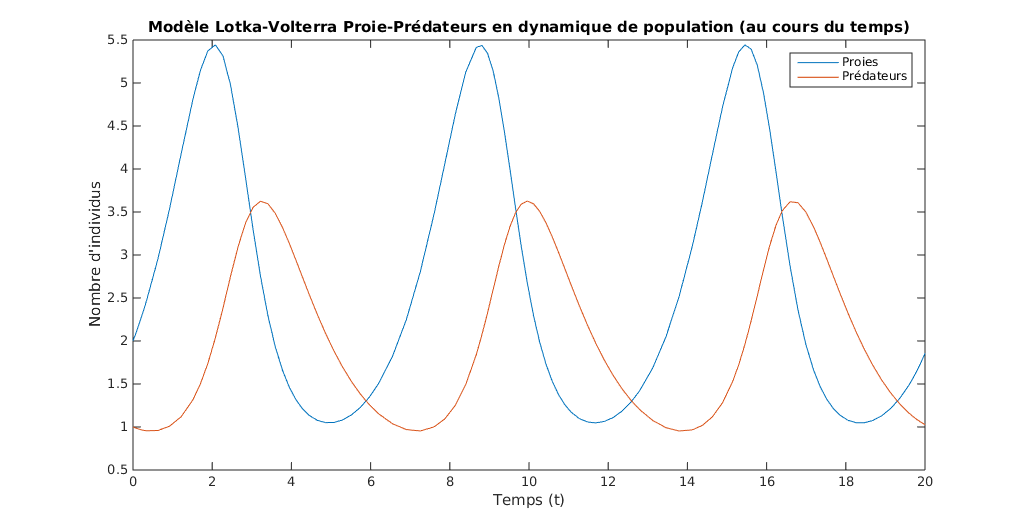
\includegraphics[scale=0.5]{ex4_EDOpredpreybis.png}}
&
\subfloat[Portait de phases des populations $y_1$ et $y_2$.]{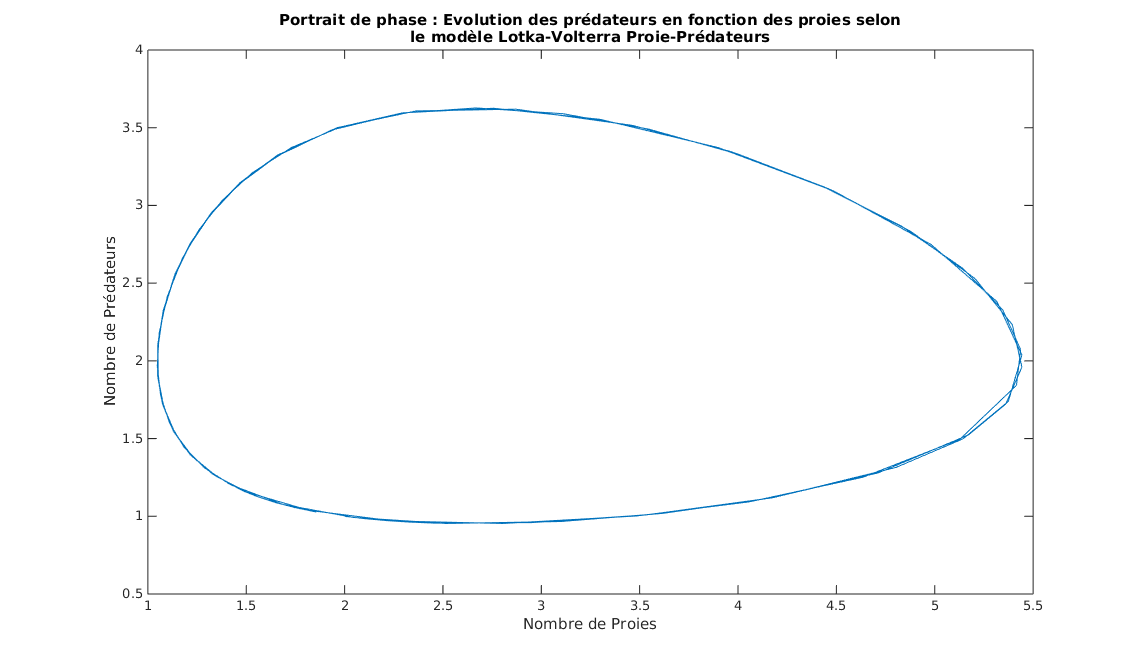
\includegraphics[scale=0.4]{ex4_EDOpredprey2.png}}
\\
\end{tabular}
\end{table}	
On remarque qu'il s'agit d'une configuration en \textbf{centres}: Les oscillations périodiques sont régulières, et le portrait de phases est une trajectoire fermée cyclique.\\
Pour savoir si ce système dynamique donne des centres, et ceci quelques soient les paramètres, ou non, on procèdera à une étude analytique de ce système.
\subsubsection{Etude Analytique}
$$
(PP)
\left \{
\begin{array}{l}
	y'_1=1.2y_1-0.6y_1y_2\\
	y'_2=-0.8y_2+0.3y_1y_2\\
	y_1(0)=2\\
	y_2(0)=1\\
\end{array}
\right.$$\\
Les équilibres vérifient $y'_1=0$ et $y'_2=0$.\\
Or, $y'_1=0\Leftrightarrow y_1=0$ ou $y_2=\frac{1.2}{0.6}=2$. De même, $y'_2=0\Leftrightarrow y_2=0$ ou $y_1=\frac{0.8}{0.3}=\frac{8}{3}$.\\

Donc \textbf{on a deux équilibres, en ${y_1 \choose y_2}={0 \choose 0}$ et ${2 \choose  8/3}$}. Pour étudier leur stabilité, on linéarise le système au voisinage des points par un développement de Taylor d'ordre 1:\\
Soit $
A=
\left(
\begin{array}{cc}
\frac{\partial y'_1}{y_1} & \frac{\partial y'_1}{y_2} \\
\frac{\partial y'_2}{y_1} & \frac{\partial y'_2}{y_2} \\
\end{array}
\right)
=
\left(
\begin{array}{cc}
1.2-0.6y_2 & -0.6y_1 \\
0.3y_2 & 0.3y_1-0.8 \\
\end{array}
\right)$ la matrice jakobienne du système. On pourra calculer sa valeur à chaque point d'équilibre, et en ces points, si $det(A|_{*})\neq0$, les portraits de phases de la linéarisation et du système sont topologiquement équivalents.
\paragraph{Au point d'équilibre $(0,0)$ :}
$A|_{(0,0)}=
\left(
\begin{array}{cc}
1.2 & 0 \\
0 & -0.8 \\
\end{array}
\right)$: On a deux valeurs propres réelles de signe opposé, $det(A|_{(0,0)})<0$, on peut donc dire que le point d'équilibre $(0,0)$ appartient à la classe d'équivalences topologiques des \textbf{points selles}.

\paragraph{Au point d'équilibre $(\frac{8}{3},2)$ :}
$A|_{\frac{8}{3},2}
\left(
\begin{array}{cc}
0&-1.6 \\
0.6&0 \\
\end{array}
\right)$: On remarque que les valeurs propres sont imaginaires pures. On a $det(A|_{(\frac{3}{8},2)})>0$ et $tr(A|_{(\frac{3}{8},2)})=0$, \textbf{la linéarisation prévoit donc des centres}, mais on ne peut rien conclure.\\

On va chercher à vérifier l'existence de centres par une intégrale première. Posons:
$$\frac{dy_2}{dy_1}=\frac{-0.8y_2+0.3y_1y_2}{1.2y_1-0.6y_1y_2}=\frac{y_2}{(1.2-0.6y_2)}\frac{(0.3y_1-0.8)}{y_1}$$
$$\frac{(0.3y_1-0.8)}{y_1}dy_1=\frac{(1.2-0.6y_2)}{y_2}dy_2$$
Intégrons, $y_1$ et $y_2$ étant positifs:
$$0.3y_1-0.8ln(y_1)=1.2ln(y_2)-0.6y_2+cte$$
Donc la fonction $H(y_1,y_2)=0.3y_1-0.8ln(y_1)-1.2ln(y_2)+0.6y_2$ est donc constante le long des trajectoires du portrait de phases, ses courbes de niveau seront les orbites du système.\\

Approximons $H(y_1,y_2)$ pour $(y_1,y_2)$ proche de $(\frac{3}{8},2)$ par un développement de Taylor à l'ordre 2:
$$H(y_1,y_2)\approx H(3/8,2)+\frac{\partial H}{\partial y_1}|_{(\frac{3}{8},2)}(y_1-\frac{3}{8})+\frac{\partial H}{\partial y_2}|_{(\frac{3}{8},2)}(y_2-2)+\frac{\partial^2 H}{\partial y_1^2}|_{(\frac{3}{8},2)}\frac{(y_1-\frac{3}{8})^2}{2!}+\frac{\partial^2 H}{\partial y_2^2}|_{(\frac{3}{8},2)}\frac{(y_2-2)^2}{2!}+\frac{\partial^2 H}{\partial y_2\partial y_1}|_{(\frac{3}{8},2)}(y_1-\frac{3}{8})(y_2-2)$$
Ce qui se réduit, quand on calcule, à 
$$H(y_1,y_2)\approx H(3/8,2)-\left[\frac{0.3^2}{2*0.8}(y_1-\frac{3}{8})^2+\frac{0.6^2}{2*1.2}(y_2-2)^2\right]$$
$$H(y_1,y_2)\approx 1.26-\left[0.056(y_1-\frac{3}{8})^2+0.15(y_2-2)^2\right]$$
Il s'agit de l'équation d'un paraboloïde centré sur $(\frac{3}{8},2)$. Ainsi, à proximité du point d'équilibre, les courbes de niveau de H sont bien fermées, et donc les orbites du système aussi, donc \textbf{on a bien de réels centres}. la simulation obtenue sur Matlab est cohérente.\\

\textbf{Le centre a pour coordonnées ${\frac{0.8}{0.3} \choose \frac{1.2}{0.6}}$ donc il dépend directement des paramètres du système.} Cependant, le centre existe tant que ces paramètres ont ces signes, donc changer leur valeur ne suffit pas à modifier la stabilité du point d'équilibre.\\
On pourrait les faire changer de signe ou les annuler, mais cette fois, on ne modéliserait plus la cohabitation entre Proies et Prédateurs \textit{(on modéliserait du commensalisme, mutualisme, ou d'autres formes d'interactions)}.\\

On peut cependant chercher à modifier la réponse fonctionnelle pour changer l'équilibre:\\
Si l'on considère que le nombre de proies mangées par prédateur tend vers un maximum asymptotique, on ne modélise plus l'effet de l'interaction par les termes  $-0.6y_1y_2$ et $+0.3y_1y_2$, mais par $-\frac{0.6y_1y_2}{1+0.6y_1}$ et $+\frac{0.3y_1y_2}{1+0.6y_1}$:
\section{Exercice 5 - Contrôler les options d'intégration}
\section{Exercice 6 - Matlab et les problèmes raides}

$(VDP)$
\[
\left\{
\begin{array}{ll}
y_1''(t)-\mu(1-y_1^{2}(t))y_1'(t)+y_1(t)=0\\
y_1(0)=y_1'(0)=1\\
\end{array}
\right.
\]

Soit $y_1'(t)=y_2(t)$, alors on obtiendra l'équation:
\[
\left\{
\begin{array}{ll}
y_2(t)=y_1'(t)\\
y_2'(t)-\mu(1-y_1^{2}(t))y_2(t)+y_1(t)=0\\
y_1(0)=y_2(0)=1\\
\end{array}
\right.
\]

Ce qui équivaut à:
\[
\left\{
\begin{array}{ll}
y_1'(t)=y_2(t)\\
y_2'(t)=\mu(1-y_1^{2}(t))y_2(t)-y_1(t)\\
y_1(0)=y_2(0)=1\\
\end{array}
\right.
\]

\end{document}
